%%%%%%%%%%%%%%%%%%%%%%%%%%%%%%%%%%%%%%%%%
% Short Sectioned Assignment
% LaTeX Template
% Version 1.0 (5/5/12)
%
% This template has been downloaded from:
% http://www.LaTeXTemplates.com
%
% Original author:
% Frits Wenneker (http://www.howtotex.com)
%
% License:
% CC BY-NC-SA 3.0 (http://creativecommons.org/licenses/by-nc-sa/3.0/)
%
%%%%%%%%%%%%%%%%%%%%%%%%%%%%%%%%%%%%%%%%%

%----------------------------------------------------------------------------------------
%	PACKAGES AND OTHER DOCUMENT CONFIGURATIONS
%----------------------------------------------------------------------------------------

\documentclass[paper=a4, fontsize=11pt]{scrartcl} % A4 paper and 11pt font size

\usepackage[margin=0.6in]{geometry}
\usepackage[utf8]{inputenc}
\usepackage[T1]{fontenc} % Use 8-bit encoding that has 256 glyphs
\usepackage{fourier} % Use the Adobe Utopia font for the document - comment this line to return to the LaTeX default
\usepackage[english]{babel} % English language/hyphenation
\usepackage{amsmath,amsfonts,amsthm} % Math packages

\usepackage{lipsum} % Used for inserting dummy 'Lorem ipsum' text into the template
\usepackage{multicol}
\usepackage{sectsty} % Allows customizing section commands
\allsectionsfont{\centering \normalfont\scshape} % Make all sections centered, the default font and small caps

\usepackage{fancyhdr} % Custom headers and footers
\pagestyle{fancyplain} % Makes all pages in the document conform to the custom headers and footers
\fancyhead{} % No page header - if you want one, create it in the same way as the footers below
\fancyfoot[L]{} % Empty left footer
\fancyfoot[C]{} % Empty center footer
\fancyfoot[R]{\thepage} % Page numbering for right footer
\renewcommand{\headrulewidth}{0pt} % Remove header underlines
\renewcommand{\footrulewidth}{0pt} % Remove footer underlines
\setlength{\headheight}{13.6pt} % Customize the height of the header
\usepackage{enumitem}
\setlist{leftmargin=40mm}
\usepackage{graphicx}

\numberwithin{equation}{section} % Number equations within sections (i.e. 1.1, 1.2, 2.1, 2.2 instead of 1, 2, 3, 4)
\numberwithin{figure}{section} % Number figures within sections (i.e. 1.1, 1.2, 2.1, 2.2 instead of 1, 2, 3, 4)
\numberwithin{table}{section} % Number tables within sections (i.e. 1.1, 1.2, 2.1, 2.2 instead of 1, 2, 3, 4)

\setlength\parindent{0pt} % Removes all indentation from paragraphs - comment this line for an assignment with lots of text

%----------------------------------------------------------------------------------------
%	TITLE SECTION
%----------------------------------------------------------------------------------------

\newcommand{\horrule}[1]{\rule{\linewidth}{#1}} % Create horizontal rule command with 1 argument of height

\title{\vspace{-1.5cm}
\normalfont \normalsize 
\textsc{Instituto Superior Técnico\\Universidade de Lisboa} \\ [12pt] % Your university, school and/or department name(s)
\huge Specification of Software 2015/16\\2\textsuperscript{nd} Project Report \\ [5pt]
}

\author{
  Daiane Oliveira\\
  \texttt{ist423160}
  \and
  Tiago Diogo\\
  \texttt{ist173559}
}

\date{\normalsize\today} % Today's date or a custom date

\begin{document}

\maketitle % Print the title

\section{Project Architecture}
This project is based on a set of signatures representing the elements of the model. Each signature can be seen as a class containing attributes, is this case, other signatures. To model the state, and allow the "passing of time" each function operates on the present instance of GitBob and return a new, changed one. The used signatures and their roles is the following:

\begin{itemize}
	\item[\textbf{Sig.Email}] A signature representing all the emails that users can register in GitBob
	\item[\textbf{Sig.User}] A signature representing all the users that can register in GitBob
	\item[\textbf{Sig.Reg\_User}] A registered user is a signature with 3 relations, to respectively, one User, one Email and one Type. A diagram of a registered user can be seen in Figure \ref{fig:reg_user}.1
	\item[\textbf{Sig.File}] A signature representing all the files than can be uploaded to GitBob
	\item[\textbf{Sig.Reg\_File}] A registered file is a signature that models the files when they are uploaded to GitBob. Is has 4 relations, one File, two Integers representing the size and version and one Reg\_User, the owner. A diagram of a registered file can be seen in Figure \ref{fig:reg_file}.2 
	\item[\textbf{Sig.Type}] An abstract class representing the profile type. It is extended by the Signatures Basic and Premium. A diagram of the Signature Type and its extensions can be seen in Figure \ref{fig:types}.3
	\item[\textbf{Sig.Basic, Premium}] The extensions of the Signature Type
	\item[\textbf{Sig.Mode}] An abstract class representing the possible sharing modes of a file. It is extended by the Signatures Regular, Secure and Readonly. A diagram of the Signature Mode can be seen in Figure \ref{fig:modes}.4
	\item[\textbf{Sig.Regular, Secure, Readonly}] The extensions of the Signature Mode
	\item[\textbf{Sig.GitBob}] This is the main signature of the model. It holds the set of registered users, the set of uploaded files and the relations that model the shares and modes of the uploaded files. This is also the signature that changes over time to allow that functions can operate over the model. The list of predicates that is allowed to change the state is defined in the fact "traces". A diagram of GitBob can be seen in Figure \ref{fig:gitbob}.5
\end{itemize}

\section{Modelling Diagrams}
\begin{figure}[h]
  \centering
  \begin{minipage}{0.4\textwidth}
    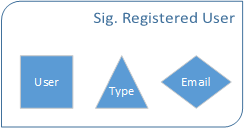
\includegraphics[width=\textwidth]{sig_reg_user.png}
    \label{fig:reg_user}
    \caption{}
  \end{minipage}
  \hfill
  \begin{minipage}{0.55\textwidth}
    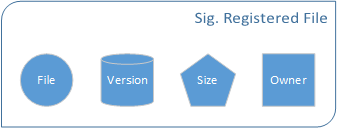
\includegraphics[width=\textwidth]{sig_reg_file.png}
    \label{fig:reg_file}
    \caption{}
  \end{minipage}
  \hfill
\end{figure}

\begin{figure}[h]
  \centering
  \begin{minipage}[b]{0.3\textwidth}
    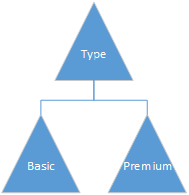
\includegraphics[width=\textwidth]{sig_types.png}
    \label{fig:types}
    \caption{}
  \end{minipage}
  \hfill
  \begin{minipage}[b]{0.45\textwidth}
    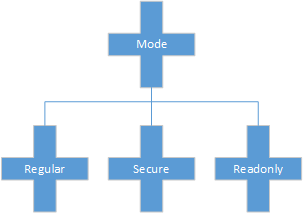
\includegraphics[width=\textwidth]{sig_modes.png}
    \label{fig:modes}
    \caption{}
  \end{minipage}
\end{figure}

\begin{figure}
\centering
 \begin{minipage}[b]{0.5\textwidth}
    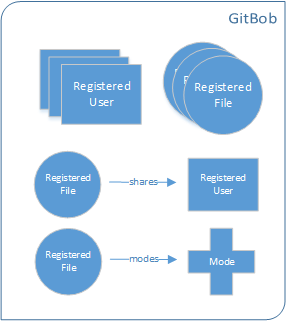
\includegraphics[width=\textwidth]{sig_gitbob.png}
    \label{fig:gitbob}
    \caption{}
  \end{minipage}
\end{figure}

\end{document}